\documentclass[11pt,a4paper]{article}
\usepackage[utf8]{inputenc}
\usepackage[T1]{fontenc}
\usepackage[french]{babel}
\frenchbsetup{StandardLists=true}
\usepackage[left=2cm,right=2cm,top=2cm,bottom=2cm]{geometry}
\usepackage[dvipsnames]{xcolor}
\usepackage{fouriernc}
\usepackage{amsmath,amssymb,amsfonts}
\usepackage{array,tabularx,booktabs,multirow}
\usepackage{colortbl}
\usepackage{graphicx}
\usepackage{mdframed}
\usepackage{enumitem}
\usepackage{fancyhdr}
\usepackage{chemformula}
\usepackage{awesomebox}
\setlength{\aweboxvskip}{0mm}
\usepackage{tcolorbox}
\tcbuselibrary{skins}
\usepackage{fontawesome5}

% ── Couleurs ──────────────────────────────────────────────────────────────────
\definecolor{exoheader}{HTML}{1E5AA0}
\definecolor{exolight}{HTML}{DCE8FF}
\definecolor{warnorange}{RGB}{220,100,0}
\definecolor{problemebg}{HTML}{FFFDE7}

% ── Tableaux ──────────────────────────────────────────────────────────────────
\renewcommand{\arraystretch}{2}
\setlength{\extrarowheight}{1mm}

% ── En-tête / pied de page (style habituel) ───────────────────────────────────
\pagestyle{fancy}
\renewcommand\headrulewidth{1pt}
\fancyhead[L]{Académie de Besançon}
\fancyhead[C]{\textbf{TP — Synthèse du benzoate de méthyle}}
\fancyhead[R]{Terminale / BTS Chimie}
\fancyfoot[C]{page \thepage}
\fancyfoot[R]{2025 -- 2026}
\fancyfoot[L]{Alexis RUIZ}

% ── Macros sections ────────────────────────────────────────────────────────────
\newcommand{\sectitle}[1]{%
  \vspace{6pt}
  \noindent\colorbox{exoheader}{\parbox{\dimexpr\linewidth-2\fboxsep}%
    {\color{white}\bfseries\large\strut\quad #1}}
  \vspace{4pt}
}
\newcommand{\subsectitle}[1]{%
  \vspace{4pt}
  \noindent\colorbox{exolight}{\parbox{\dimexpr\linewidth-2\fboxsep}%
    {\color{exoheader}\bfseries\strut\quad #1}}
  \vspace{2pt}
}

% ── Macro question ────────────────────────────────────────────────────────────
\newcounter{question}
\newcommand{\question}{%
  \stepcounter{question}%
  \noindent\textcolor{exoheader}{\textbf{Question \thequestion.}}\quad
}

% ── Disque bleu pour exercice de correspondance ───────────────────────────────
\newcommand{\disque}{\textcolor{exoheader}{\large\textbullet}}

\begin{document}

% ── En-tête élève ─────────────────────────────────────────────────────────────
\noindent\textbf{NOM :}\hfill\textbf{Prénom :}\hfill\textbf{Classe :}\hfill\phantom{x}\\[0.2cm]
\hrule
\vspace{0.2cm}

\begin{center}
  {\large\bfseries\textcolor{exoheader}{Travaux Pratiques de Chimie Organique}}\\[4pt]
  {\LARGE\bfseries Synthèse du benzoate de méthyle}\\[2pt]
  {\small Académie de Besançon — Belfort}
\end{center}
\hrule
\vspace{6pt}

% ── Problématique ─────────────────────────────────────────────────────────────
\begin{tcolorbox}[
  enhanced,
  colback=problemebg,
  colframe=exoheader,
  boxrule=1.5pt,
  title={\faFlask\quad Problématique},
  fonttitle=\bfseries\color{white},
  attach boxed title to top left={yshift=-2mm, xshift=4mm},
  boxed title style={colback=exoheader, colframe=exoheader}
]
\textit{Une parfumeure reçoit une commande urgente de benzoate de méthyle, l'arôme
caractéristique de la goyave indispensable à la fabrication de son nouveau parfum.
Ses stocks sont épuisés et son fournisseur ne peut pas livrer avant plusieurs semaines.
\textbf{Peut-elle synthétiser elle-même cet ester en laboratoire à partir de réactifs
disponibles, et comment s'assurer de sa pureté ?}}
\end{tcolorbox}

\vspace{4pt}
\begin{mdframed}[backgroundcolor=exolight, linecolor=exoheader, linewidth=1.2pt]
Le \textbf{benzoate de méthyle} (\ch{C6H5COOCH3}) est utilisé en parfumerie pour son odeur de
goyave. C'est un liquide qui bout à \textbf{199°C}, obtenu par réaction de l'acide benzoïque
avec le méthanol en présence d'ions \ch{H+}.
\end{mdframed}

\vspace{6pt}

% ══════════════════════════════════════════════════════════════════════════════
\sectitle{Partie I — Étude de la réaction de synthèse}
% ══════════════════════════════════════════════════════════════════════════════

\subsectitle{1. Identification des espèces chimiques}

\question À l'aide du tableau en annexe, compléter le tableau suivant :

\vspace{4pt}
\begin{center}
\begin{tabularx}{\linewidth}{|>{\centering\bfseries\color{white}\columncolor{exoheader}}m{2.6cm}
                              |>{\centering\arraybackslash}m{1.8cm}
                              |>{\centering\arraybackslash}m{2cm}
                              |>{\centering\arraybackslash}m{3cm}
                              |>{\centering\arraybackslash}X
                              |>{\centering\arraybackslash}m{1.5cm}
                              |>{\centering\arraybackslash}m{2cm}|}
\hline
\rowcolor{exoheader}
\color{white}Nom & \color{white}Famille & \color{white}Groupe caract. &
\color{white}Formule développée & \color{white}Formule semi-dév. &
\color{white}Formule brute & \color{white}Modèle mol. \\
\hline
Acide benzoïque & & &
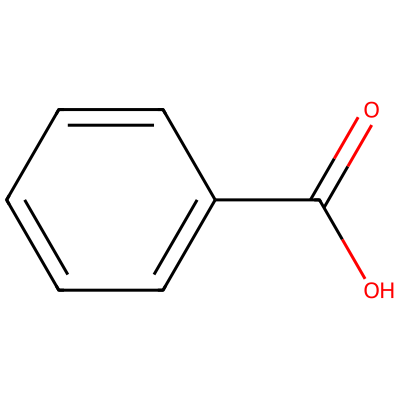
\includegraphics[width=2.8cm]{2d_acide_benzoique.png} & & &
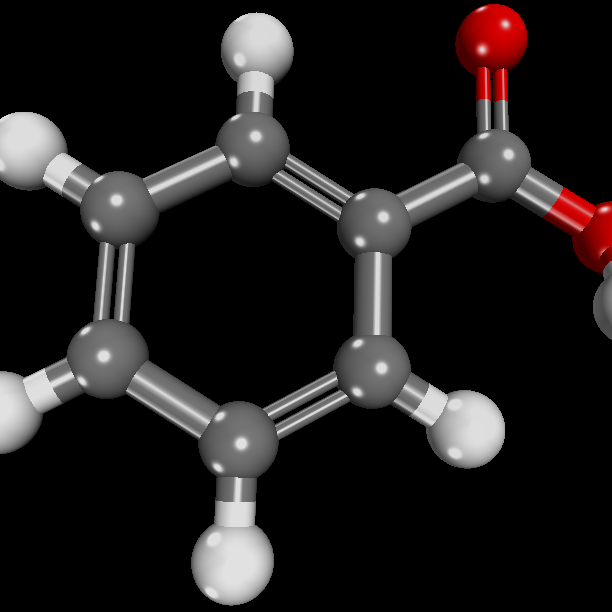
\includegraphics[width=1.9cm]{acide_benzoique.png} \\
\hline
Méthanol & & &
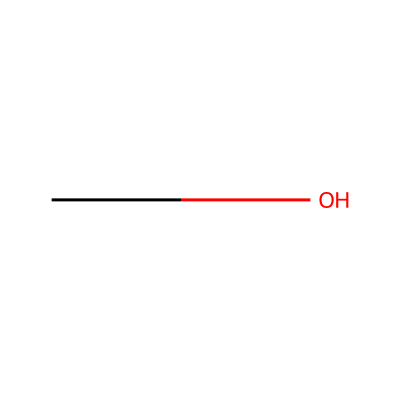
\includegraphics[width=1.8cm]{2d_methanol.png} & & &
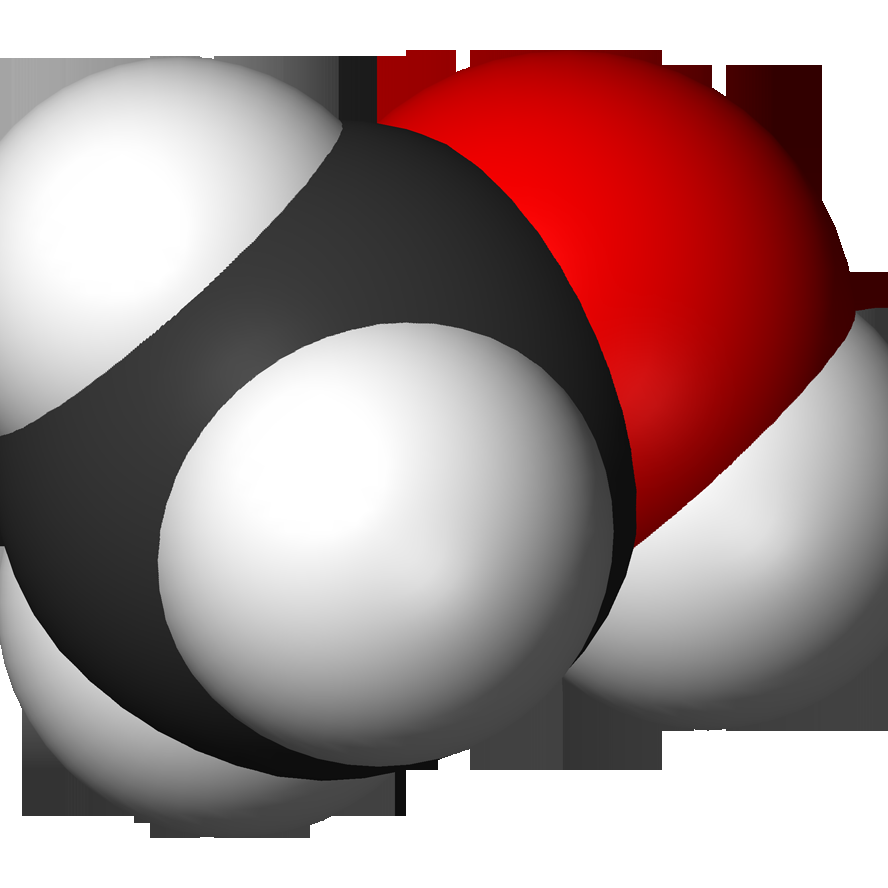
\includegraphics[width=1.5cm]{methanol.png} \\
\hline
Benzoate de méthyle & & &
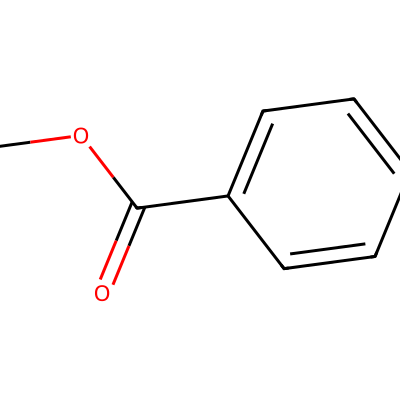
\includegraphics[width=2.8cm]{2d_benzoate_methyle.png} &
\ch{C6H5COOCH3} & \ch{C8H8O2} &
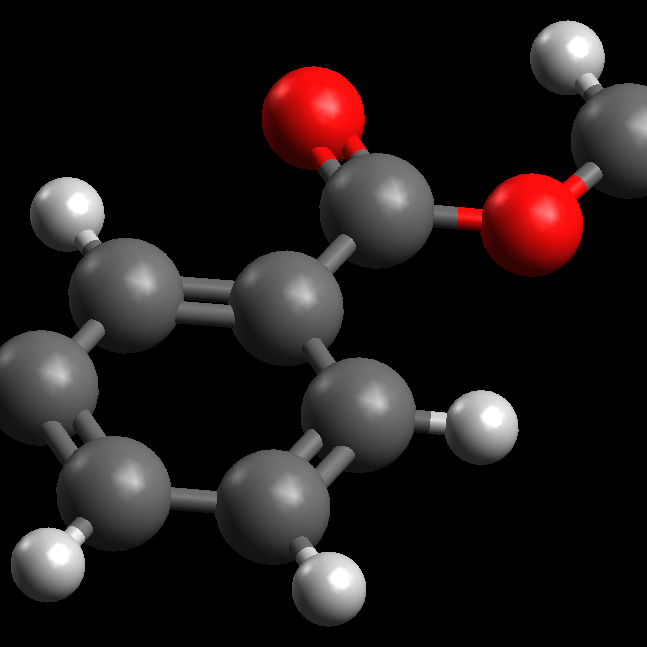
\includegraphics[width=1.9cm]{Methyl_Benzoate_3D_Computer_Model.png} \\
\hline
\end{tabularx}
\end{center}

\vspace{6pt}
\subsectitle{2. Équation de la réaction}

L'équation de la réaction modélisant cette transformation chimique est :

\vspace{4pt}
\begin{center}
\begin{tabularx}{0.92\linewidth}{|>{\centering\arraybackslash\columncolor{exolight}}X
                                  |>{\centering\arraybackslash\columncolor{exolight}}m{0.6cm}
                                  |>{\centering\arraybackslash\columncolor{exolight}}X
                                  |>{\centering\arraybackslash\columncolor{exolight}}m{1.2cm}
                                  |>{\centering\arraybackslash\columncolor{exolight}}X
                                  |>{\centering\arraybackslash\columncolor{exolight}}m{0.6cm}
                                  |>{\centering\arraybackslash\columncolor{exolight}}X|}
\hline
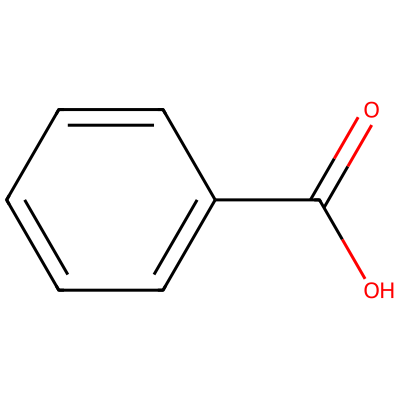
\includegraphics[width=2.2cm]{2d_acide_benzoique.png} &
\textbf{+} &
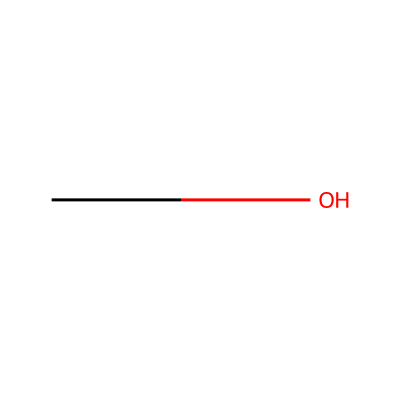
\includegraphics[width=1.5cm]{2d_methanol.png} &
$\overset{\ch{H+}}{\rightleftharpoons}$ &
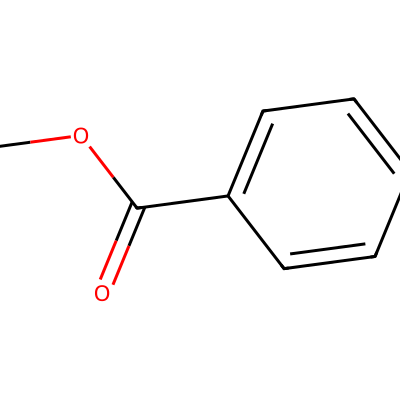
\includegraphics[width=2.2cm]{2d_benzoate_methyle.png} &
\textbf{+} &
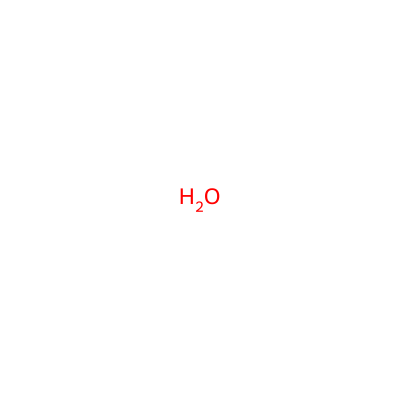
\includegraphics[width=1.2cm]{2d_eau.png} \\
Acide benzoïque & & Méthanol & & Benzoate de méthyle & & Eau \\
\hline
\end{tabularx}
\end{center}

\vspace{4pt}
\question Compléter sur les pointillés la formule du dernier produit ainsi que son nom.

\vspace{4pt}
\question Quel nom porte cette réaction ? \dotfill

\vspace{6pt}

% ══════════════════════════════════════════════════════════════════════════════
\sectitle{Partie II — Mode opératoire}
% ══════════════════════════════════════════════════════════════════════════════

\subsectitle{1. Ordre chronologique du protocole}

\question Les étapes du protocole sont dans le désordre. Retrouver l'ordre chronologique
en reliant chaque étape (colonne gauche) à sa description (colonne droite).

\vspace{4pt}
\begin{center}
\begin{tabularx}{\linewidth}{@{}m{1.6cm}
                              @{\hspace{2pt}}>{\centering\arraybackslash}m{0.5cm}
                              @{\hspace{6pt}}
                              >{\centering\arraybackslash}m{0.5cm}@{\hspace{2pt}}
                              X@{}}
\rowcolor{exoheader}
\color{white}\bfseries Étape &
\color{white}\bfseries \disque &
\color{white}\bfseries \disque &
\color{white}\bfseries Description \\[2pt]
Étape 1 & \disque & \disque & Chauffer à reflux pendant 1 heure à ébullition douce. \\[6pt]
Étape 2 & \disque & \disque & Introduire 12,2 g d'acide benzoïque, 40 mL de méthanol, 3 gouttes d'acide sulfurique concentré et quelques grains de pierre ponce dans un ballon. \\[6pt]
Étape 3 & \disque & \disque & Agiter en dégazant ; séparer les deux phases et garder la phase organique. \\[6pt]
Étape 4 & \disque & \disque & Verser après refroidissement dans une ampoule à décanter avec 50 mL d'eau salée saturée. \\[6pt]
Étape 5 & \disque & \disque & Sécher avec du sulfate de cuivre anhydre, filtrer et recueillir le filtrat. \\[6pt]
Étape 6 & \disque & \disque & Ajouter 60 mL d'hydrogénocarbonate de sodium à 5\%, dégazer et séparer les phases. \\[6pt]
\end{tabularx}
\end{center}

\vspace{6pt}
\subsectitle{2. Pictogrammes de sécurité}

\question On a relevé les pictogrammes de sécurité des réactifs.
Relier chaque pictogramme à son nom et indiquer les précautions à prendre.

\vspace{4pt}
\begin{center}
\begin{tabularx}{\linewidth}{@{}>{\centering\arraybackslash}m{2.2cm}
                              @{\hspace{4pt}}>{\centering\arraybackslash}m{0.6cm}
                              @{\hspace{1cm}}
                              >{\centering\arraybackslash}m{0.6cm}@{\hspace{4pt}}
                              X@{}}
\rowcolor{exoheader}
\color{white}\bfseries Pictogramme &
\color{white}\bfseries \disque &
\color{white}\bfseries \disque &
\color{white}\bfseries Nom / Précautions \\[4pt]

\includegraphics[width=1.8cm]{inflammable.png} & \disque & \disque & \dotfill \\[1cm]
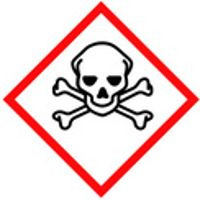
\includegraphics[width=1.8cm]{toxique.png}     & \disque & \disque & \dotfill \\[1cm]
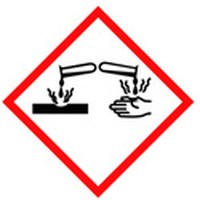
\includegraphics[width=1.8cm]{corrosif.png}    & \disque & \disque & \dotfill \\[1cm]

\includegraphics[width=1.8cm]{nocif.png}       & \disque & \disque & \dotfill \\[1cm]
\end{tabularx}
\end{center}

\newpage
% ══════════════════════════════════════════════════════════════════════════════
\sectitle{Partie III — Protocole expérimental}
% ══════════════════════════════════════════════════════════════════════════════

\begin{mdframed}[backgroundcolor=orange!15, linecolor=warnorange, linewidth=2pt]
\textbf{\textcolor{warnorange}{\faExclamationTriangle\quad ATTENTION}} —
La manipulation des acides concentrés (acide sulfurique) nécessite
\textbf{lunettes} et \textbf{gants de protection}.
\end{mdframed}

\vspace{4pt}
\subsectitle{I — Synthèse du benzoate de méthyle}

\begin{center}
  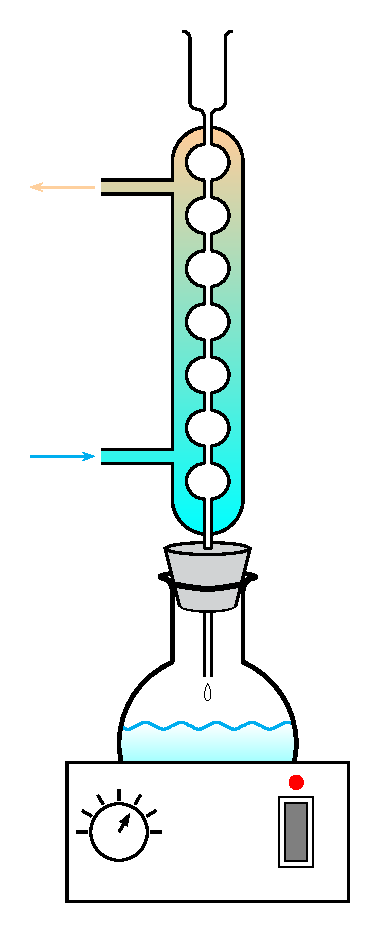
\includegraphics[height=7cm]{schema_reflux.png}\\[2pt]
  \textit{\small Montage de chauffage à reflux}
\end{center}

\begin{enumerate}[leftmargin=1.5cm, label=\textcolor{exoheader}{\textbf{\arabic*.}}]
  \item Dans un ballon de 250 mL, introduire :
    \begin{itemize}
      \item \textbf{12,2 g} d'acide benzoïque en poudre (peser précisément),
      \item \textbf{40 mL} de méthanol (éprouvette graduée),
      \item \textbf{3 gouttes} d'acide sulfurique concentré (pipette + propipette),
      \item quelques grains de \textbf{pierre ponce}.
    \end{itemize}
  \item Alimenter le réfrigérant en eau (\textit{ouvrir très progressivement le robinet})
        et porter à \textbf{ébullition douce pendant 60 minutes}.
  \item Arrêter le chauffage, abaisser le chauffe-ballon.
        Laisser refroidir à l'air ambiant puis dans un bain d'eau froide.
\end{enumerate}

\vspace{4pt}
\subsectitle{II — Extraction de l'ester}

\begin{center}
  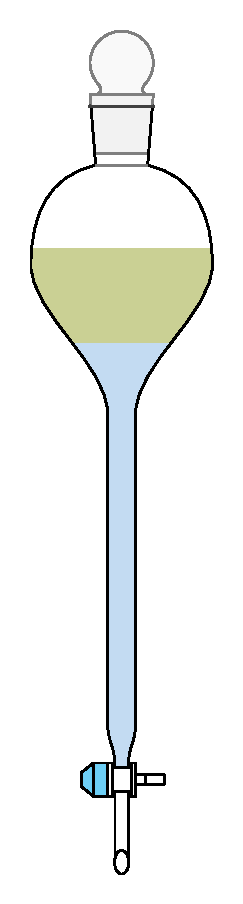
\includegraphics[height=6cm]{schema_ampoule.png}\\[2pt]
  \textit{\small Ampoule à décanter}
\end{center}

\begin{enumerate}[leftmargin=1.5cm, label=\textcolor{exoheader}{\textbf{\arabic*.}}]
  \item Verser dans une ampoule à décanter contenant \textbf{50 mL} d'eau salée saturée
        (\textit{retenir les grains de pierre ponce}).
  \item Agiter doucement en dégazant régulièrement. Attendre deux phases distinctes.

  \vspace{4pt}
  \question Identifier les deux phases à l'aide du tableau de données :
  \begin{itemize}
    \item Phase supérieure : \dotfill
    \item Phase inférieure : \dotfill
  \end{itemize}

  \item Éliminer la phase inférieure dans un bécher.
  \item Ajouter \textbf{60 mL} d'hydrogénocarbonate de sodium à 5\%.
        Agiter prudemment (\textit{dégazage violent}),
        séparer et éliminer la phase inférieure.
  \item Ajouter du \textbf{sulfate de cuivre anhydre}, filtrer,
        recueillir le filtrat dans un erlenmeyer propre et sec.
\end{enumerate}

\vspace{6pt}
\begin{mdframed}[backgroundcolor=exolight, linecolor=exoheader, linewidth=1.2pt]
\textbf{Bilan de la problématique :} \\
La parfumeure a-t-elle pu obtenir le benzoate de méthyle en laboratoire ?
Justifiez en expliquant le rôle de chaque étape d'extraction. \dotfill

\noindent\dotfill

\noindent\dotfill
\end{mdframed}

% ══════════════════════════════════════════════════════════════════════════════
\newpage
\sectitle{Annexe — Données sur les espèces chimiques}
% ══════════════════════════════════════════════════════════════════════════════

\vspace{4pt}
\subsectitle{Tableau 1 — Familles de composés organiques}

\begin{center}
\begin{tabularx}{\linewidth}{|>{\columncolor{exoheader}\color{white}\bfseries\centering\arraybackslash}m{2.5cm}
                              |>{\centering\arraybackslash}m{1.8cm}
                              |>{\centering\arraybackslash}m{1.6cm}
                              |>{\centering\arraybackslash}m{3cm}
                              |>{\centering\arraybackslash}X
                              |>{\centering\arraybackslash}m{1.4cm}
                              |>{\centering\arraybackslash}m{2cm}|}
\hline
\rowcolor{exoheader}
\color{white}Famille & \color{white}Groupe caract. & \color{white}Nom &
\color{white}Formule développée & \color{white}Formule semi-dév. &
\color{white}Formule brute & \color{white}Modèle mol. \\
\hline
Alcool & \ch{-OH} & Éthanol &
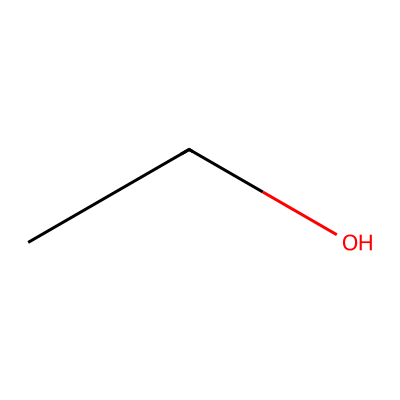
\includegraphics[width=2.8cm]{2d_ethanol.png} &
\ch{CH3-CH2-OH} & \ch{C2H6O} & 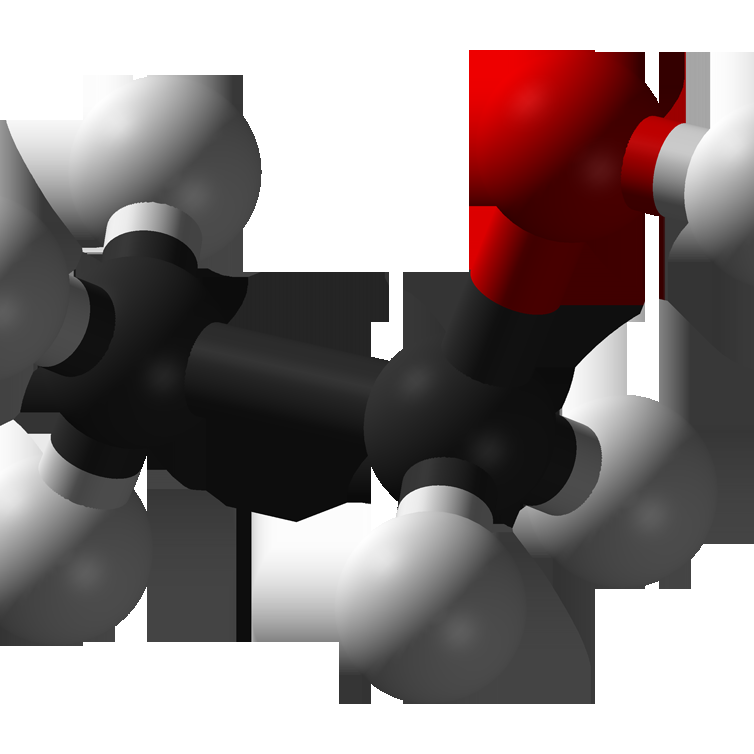
\includegraphics[width=1.8cm]{ethanol.png} \\
\hline
Cétone & \ch{-COR} & Butanone &
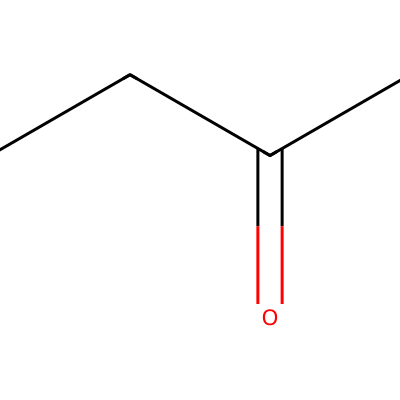
\includegraphics[width=2.8cm]{2d_butanone.png} &
\ch{CH3-CO-CH2-CH3} & \ch{C4H8O} & \\
\hline
Aldéhyde & \ch{-CHO} & Propanal &
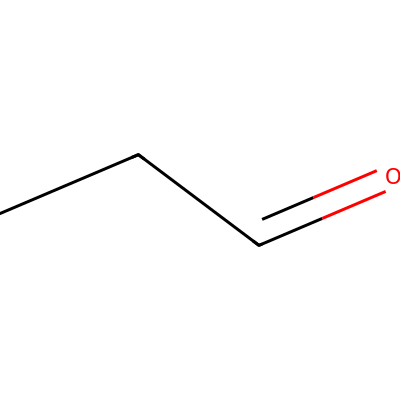
\includegraphics[width=2.8cm]{2d_propanal.png} &
\ch{CH3-CH2-CHO} & \ch{C3H6O} & 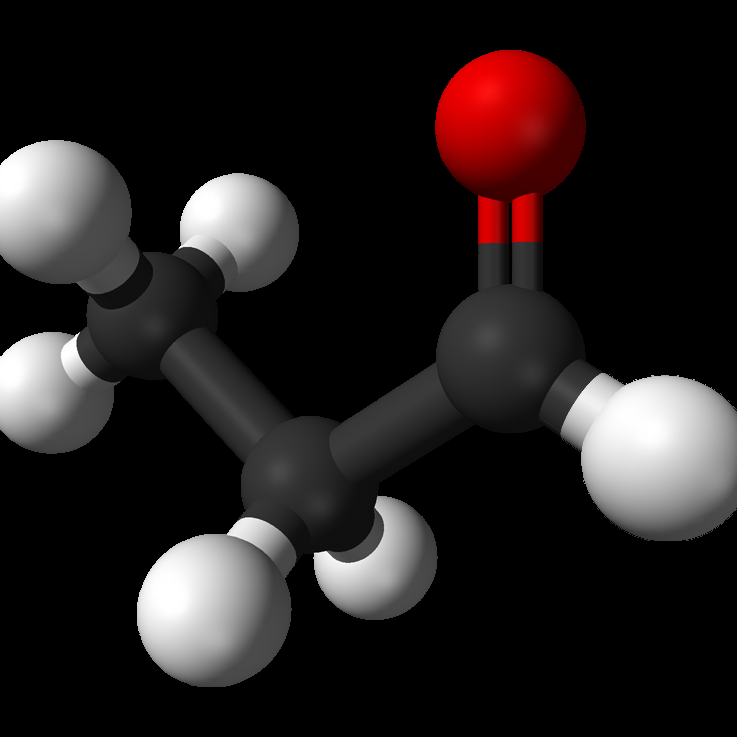
\includegraphics[width=1.8cm]{propanal.png} \\
\hline
Ester & \ch{-COOR} & Éthanoate de méthyle &
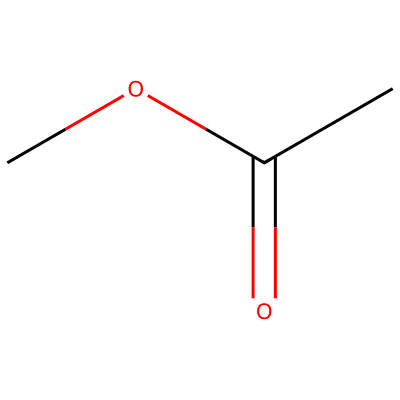
\includegraphics[width=2.8cm]{2d_ethanoate_methyle.png} &
\ch{CH3-COO-CH3} & \ch{C3H6O2} & 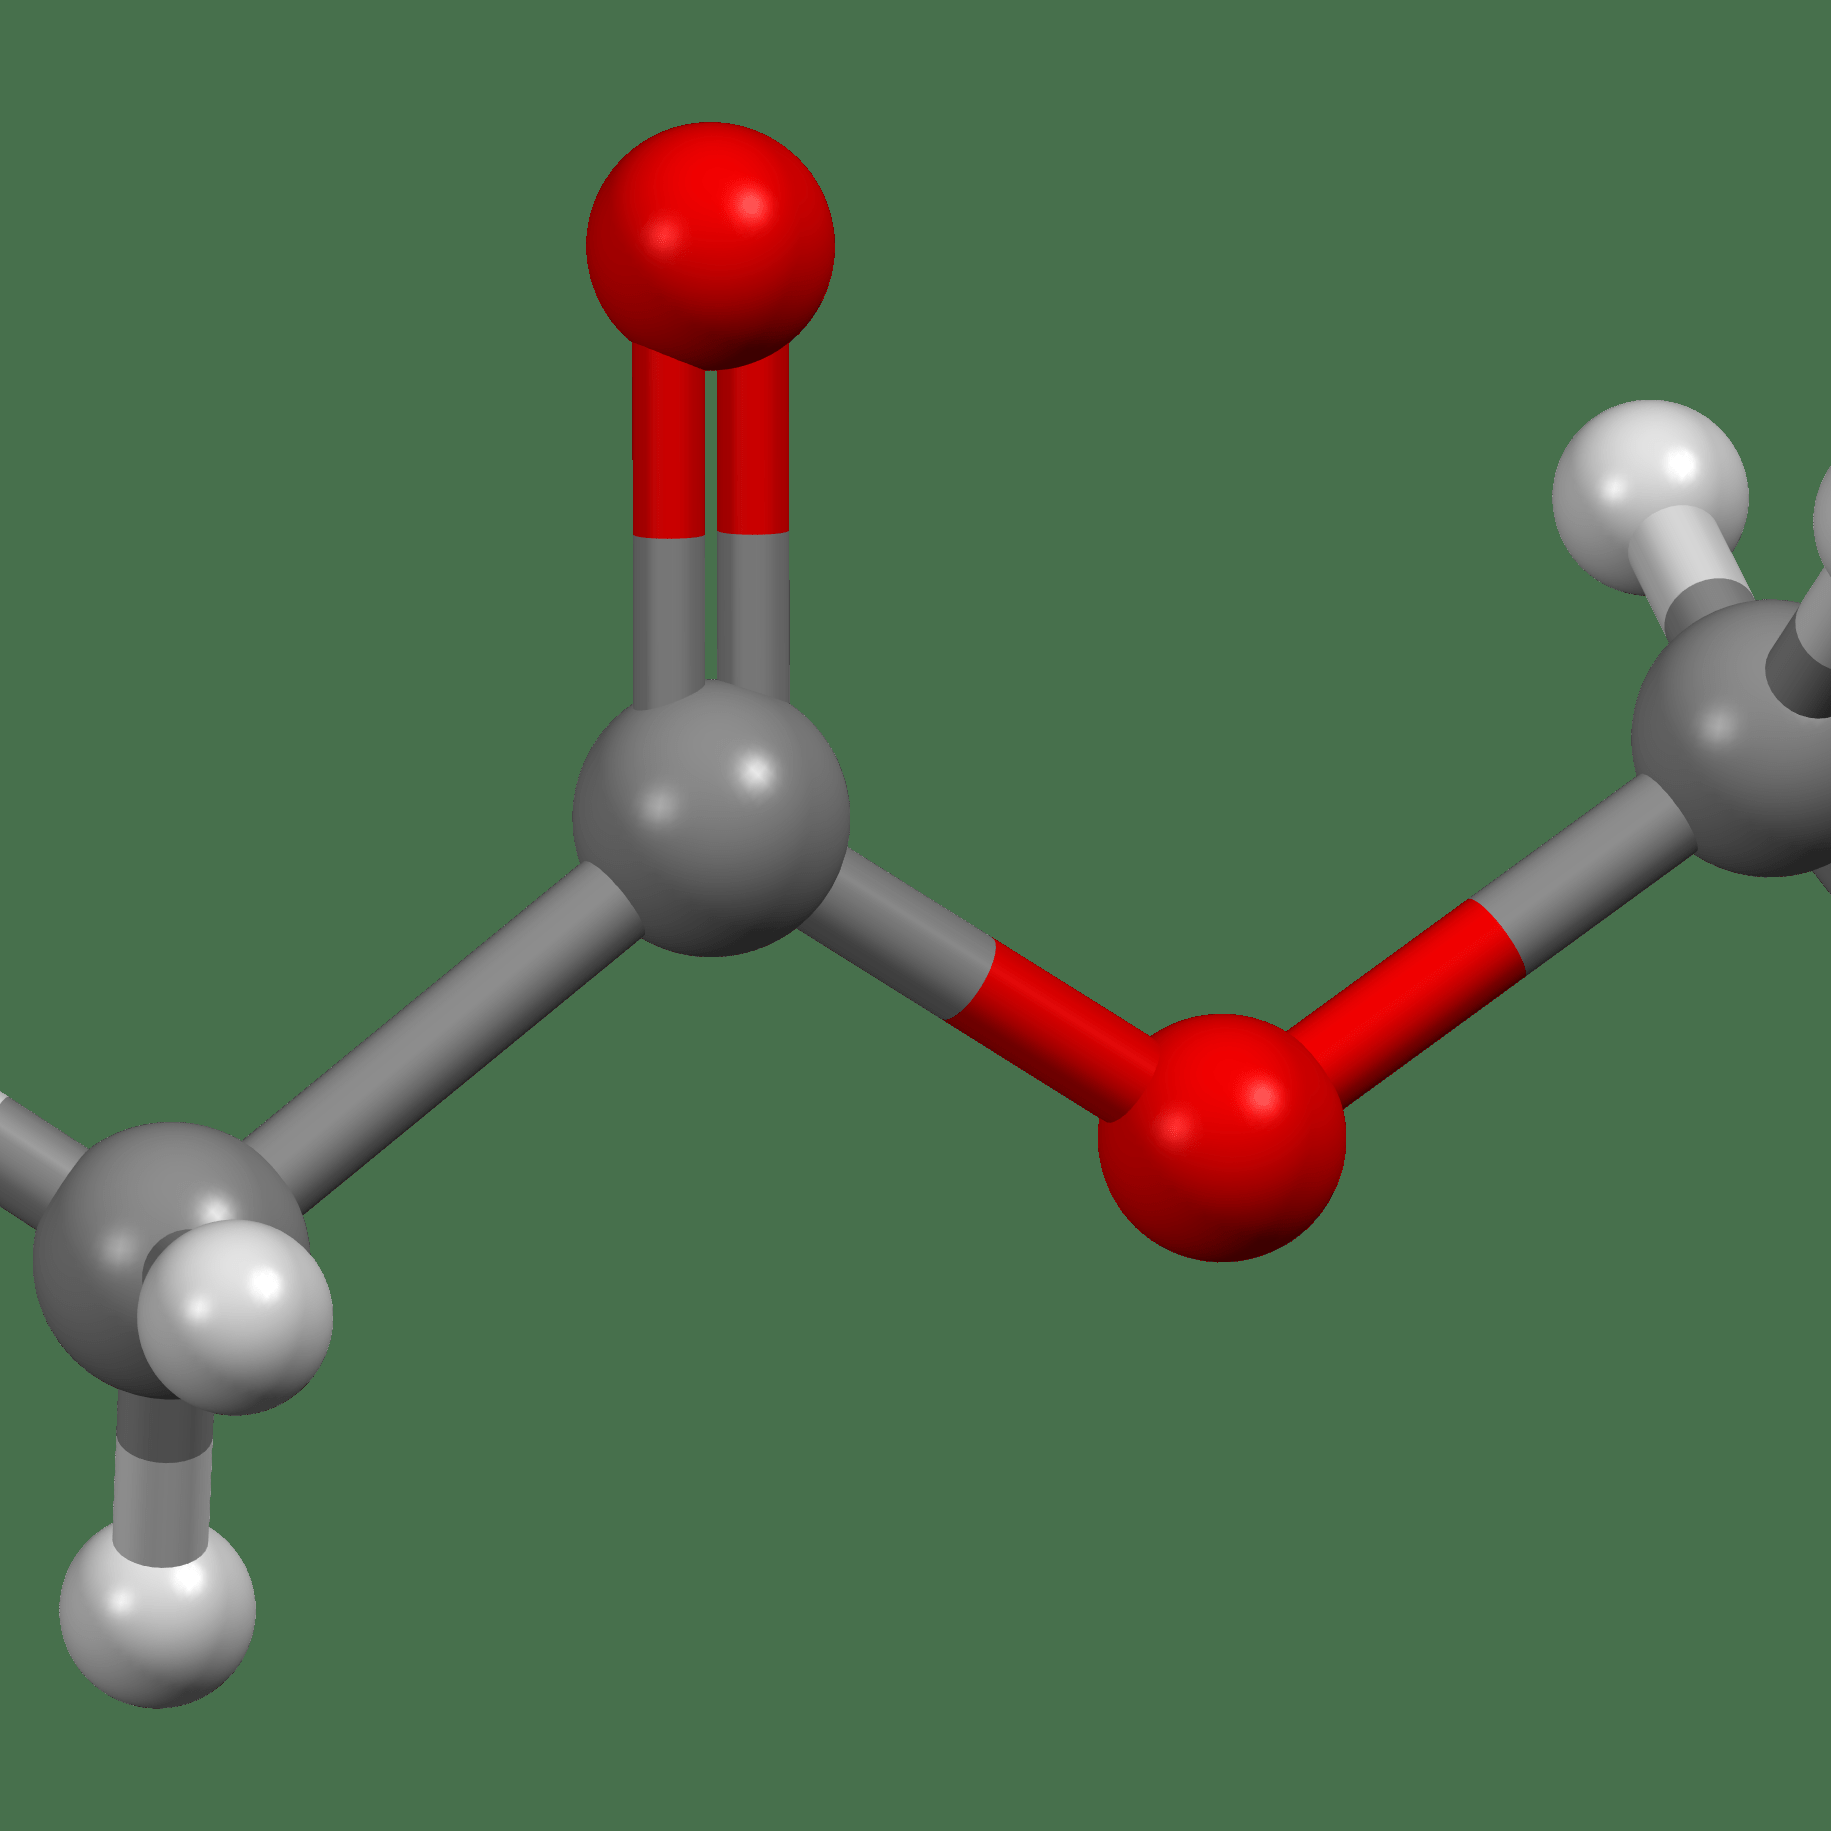
\includegraphics[width=1.8cm]{ethanoate_methyle.png} \\
\hline
Acide carboxylique & \ch{-COOH} & Acide éthanoïque &
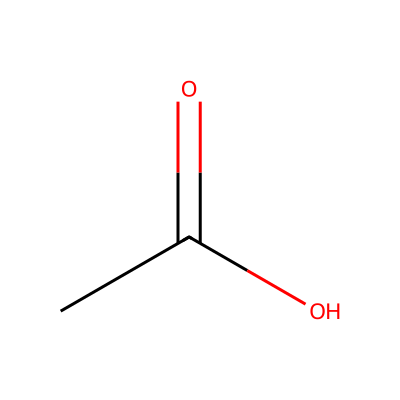
\includegraphics[width=2.8cm]{2d_acide_ethanoique.png} &
\ch{CH3-COOH} & \ch{C2H4O2} & 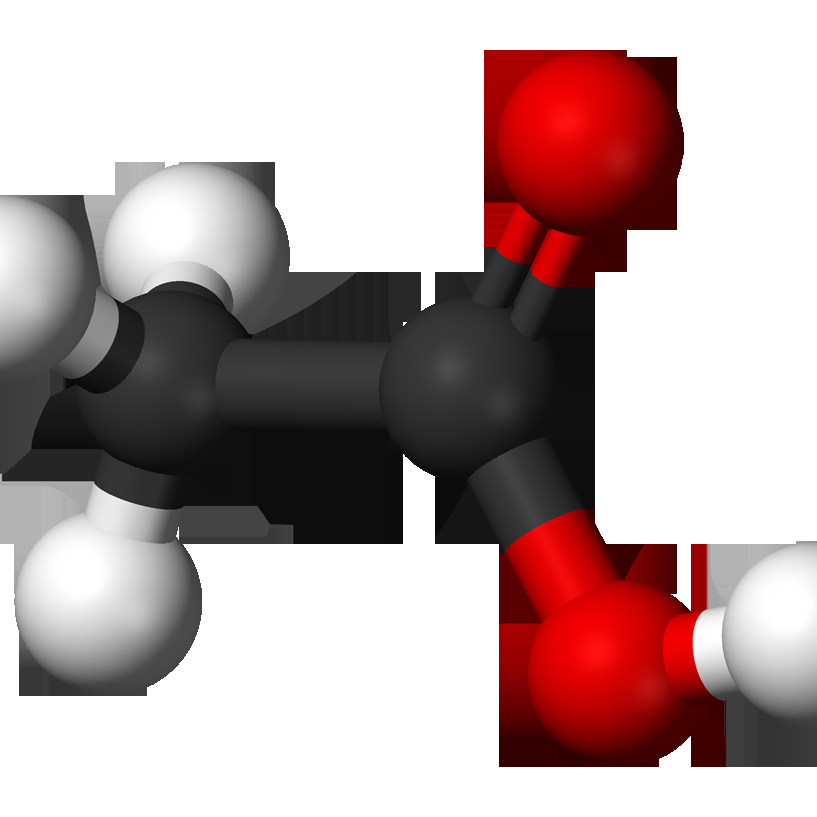
\includegraphics[width=1.8cm]{acide_ethanoique.png} \\
\hline
\end{tabularx}
\end{center}

\vspace{8pt}
\subsectitle{Tableau 2 — Caractéristiques des réactifs et produits}

\begin{center}
\begin{tabularx}{\linewidth}{|>{\columncolor{exoheader}\color{white}\bfseries\centering\arraybackslash}m{3cm}
                              |>{\centering\arraybackslash}X
                              |>{\centering\arraybackslash}X
                              |>{\centering\arraybackslash}X
                              |>{\centering\arraybackslash}X|}
\hline
\rowcolor{exoheader}
\color{white}Espèce chimique & \color{white}Acide benzoïque &
\color{white}Méthanol & \color{white}Benzoate de méthyle & \color{white}Eau salée \\
\hline
Formule brute & \ch{C7H6O2} & \ch{CH4O} & \ch{C8H8O2} & \\
\hline
Masse volumique (g/mL) & — & 0,79 & 1,1 & 1,2 \\
\hline
Solubilité dans l'eau & Très faible & Très grande & Très faible & — \\
\hline
Solubilité dans l'eau salée & Très faible & Très grande & Insoluble & — \\
\hline
Pictogrammes de sécurité & & & & \\[1cm]
\hline
\end{tabularx}
\end{center}

\end{document}
